%% =====================================================================
%%  COS 802 Research Report
%%  Business-Aware Customer Segmentation: A Comparative Evaluation of
%%  Standard, RFM-Based and Constrained K-Means Clustering
%%
%%  Template : IEEEtran (conference mode, two-column)
%%  Structure: SIGKDD Explorations research-report layout
%%             (Abstract, Keywords, Introduction, Related Work, Data,
%%              Methodology, Experiments & Results, Discussion,
%%              Conclusion & Future Work, Reproducibility, References)
%%  Results  : every number in this report was produced by an independent
%%             re-run of the project notebook on the original UCI file
%%             (Online Retail.xlsx, 541,909 rows), extended with k-selection,
%%             cross-space validation, bootstrap confidence intervals,
%%             outlier-robust effect sizes and baseline constraint rates.
%%  Compile  : pdfLaTeX. Figures are pre-rendered PDFs in figures/;
%%             their pgfplots sources are in figures/src/ (compile each
%%             with pdflatex and copy the PDF up one level to change one).
%% =====================================================================
\documentclass[conference,10pt]{IEEEtran}
\IEEEoverridecommandlockouts

% ---------- Packages ----------
\usepackage[utf8]{inputenc}
\usepackage[T1]{fontenc}
\usepackage{cite}
\usepackage{amsmath,amssymb,amsfonts}
\usepackage{graphicx}
\usepackage{textcomp}
\usepackage{xcolor}
\usepackage{booktabs}
\usepackage{multirow}
\usepackage{array}
\usepackage{algorithm}
\usepackage{algpseudocode}
\usepackage{url}
\usepackage[hidelinks]{hyperref}

% ---------- Colour-blind-safe palette ----------
\definecolor{cStd}{RGB}{0,114,178}    % Standard K-means
\definecolor{cRFM}{RGB}{230,159,0}    % RFM K-means
\definecolor{cCon}{RGB}{0,158,115}    % Constrained K-means
\definecolor{cML}{RGB}{213,94,0}      % must-link
\definecolor{cCL}{RGB}{86,180,233}    % cannot-link
% segment archetypes (PCA figure)
\definecolor{aHigh}{RGB}{213,94,0}
\definecolor{aReg}{RGB}{0,114,178}
\definecolor{aOcc}{RGB}{0,158,115}
\definecolor{aLap}{RGB}{160,160,160}

\newcommand{\etasq}{\eta^{2}}
\newcolumntype{L}[1]{>{\raggedright\arraybackslash}p{#1}}

\begin{document}

% =====================================================================
\title{CUSTOMER SEGMENTATION AND
BEHAVIOURAL ANALYSIS: A Comparison of
clustering methods for e-commerce segmentation}

\author{\IEEEauthorblockN{Nqobile Ngidi}
\IEEEauthorblockA{\textit{Student number: u15189181}\\
\textit{COS 802 Research Project, Department of Computer Science}\\
\textit{University of Pretoria}, Pretoria, South Africa\\
u15189181@tuks.co.za}}

\maketitle

% =====================================================================
\begin{abstract}
Customer segmentation is a widely used approach
in the identification of customer purchase behaviours. These
segments are used to support business decisions relating to
marketing, resource allocation and product development. However, conventional customer segmentation does not explicitly
reflect some business metrics. This study compares standard
K-means, K-means on Recency-Frequency-Monetary (RFM), and a
soft constrained K-means using the UCI Online Retail dataset.
Segments were built using historic transaction data and evaluated
against outcomes in a subsequent 90-day period that was reserved
as a temporal holdout. The model performance was measured
using Silhouette, Davies–Bouldin and Calinski–Harabasz indices,
and eta-squared measured the future business-metric separation; constraint violation rates and sensitivity analyses were also reported. The
results show that RFM K-means achieved the best internal
scores (Silhouette 0.370) and the largest future-order separation
($\eta^2 = 0.192$ versus 0.147; bootstrap 95\% CI of the difference
[0.020, 0.086]). Constrained K-means changed the assignment
of only 48 customers (1.4\%) relative to standard K-means,
raised future-order $\eta^2$ by 0.006 and lowered it in two of five
resampled constraint sets, exhibiting only marginal improvements.
The study demonstrates the importance of evaluating customer
segmentation through both statistical validity and future business
relevance. It concludes that, within the experimental setting,
RFM-based K-means provides the strongest overall performance,
while the tested country-based constraints do not establish
a meaningful advantage over standard K-means. The study
contributes a reproducible, temporally validated framework that
evaluates validity, business-oriented metrics and constraint
sensitivity.
\end{abstract}

\begin{IEEEkeywords}
customer segmentation, K-means, RFM analysis, constrained clustering,
must-link and cannot-link constraints, temporal holdout, cluster validation,
bootstrap, e-commerce analytics
\end{IEEEkeywords}

% =====================================================================
\section{Introduction}
\label{sec:intro}

\subsection{Context and motivation}
The growth of e-commerce sales has brought with it a significant expansion in e-commerce retailer data, which includes information such as customer transaction date, product type, quantity, price and unique customer identifier. These features can be used to identify customer purchase behaviours and segments, describing how often customers purchase and an estimated purchase spend. Customer segmentation has the ability to
group customers with similar behaviour so that communication, retention
effort and service levels can be tailored to each group
\cite{chen2012rfm,salminen2023algorithms}. Because transactional datasets rarely
contain segment labels, segmentation is usually framed as unsupervised
clustering \cite{wani2024comprehensive,gomes2023review}.

K-means is the most widely used model for customer segmentation; it is advantageous because it is simple to compute and
fast
\cite{macqueen1967some,gomes2023review,salminen2023algorithms}. In e-commerce it is commonly used with
the RFM framework \cite{chen2012rfm,christy2021rfm}. A further
option is constrained (semi-supervised) clustering, in which domain knowledge
is injected as pairwise must-link and cannot-link constraints
\cite{wagstaff2001constrained,basu2004probabilistic}. However, internal clustering and business relevance may not always be equivalent. A model may effectively segment customers according to recency, frequency and monetary spend but may overlook other segments that are informed by business such as geographic location.

\subsection{Problem statement}
Past studies on segmentation typically evaluate clustering by internal indices
such as the Silhouette score \cite{rousseeuw1987silhouettes}. These metrics indicate how well separated groups are in the clustering feature space, but they do not speak to separation in terms of behaviour that matters to the
business \cite{salminen2023algorithms}. Constrained
clustering is an approach that can be used to make segments ``business-aware''; however, its benefit
depends on the quality of the constraints and on how strongly they are enforced. 

Clustering methods should not only be evaluated on internal cluster separation but should be evaluated in relation to business-relevant behaviour. 

\subsection{Research questions}
\textbf{RQ1.} How does the performance of standard K-means clustering
statistically compare with RFM-based K-means and constrained K-means
clustering in customer segmentation?

\textbf{RQ2.} How does constrained clustering measurably improve
business-metric separation relative to unconstrained clustering?

RQ2 is analysed as the difference in $\etasq$ between constrained and
standard K-means, which share a feature space. This makes the comparison
measurable.

\subsection{Contributions}
\begin{enumerate}
  \item A controlled comparison of standard, RFM and soft constrained K-means
  at a common $k$.
  \item A temporal-holdout evaluation of five future outcomes.
  \item An explicit audit of the constrained model: violation rates compared
  with unconstrained and chance baselines and penalty-weight sensitivity.
\end{enumerate}

Section~\ref{sec:related} reviews related work, Section~\ref{sec:data}
describes the data and Section~\ref{sec:method} the methodology.
Section~\ref{sec:results} reports the experiments, Section~\ref{sec:discussion}
discusses them, and Section~\ref{sec:conclusion} concludes.

% =====================================================================
\section{Related Work}
\label{sec:related}

\subsection{RFM-based customer segmentation}
The RFM framework originates in database marketing and
remains the most common representation for transaction-based segmentation
\cite{gomes2023review} because each dimension is directly interpretable. Chen et~al.\
\cite{chen2012rfm} applied RFM with K-means and decision trees to the same
UK online gift retailer used here and profiled the clusters into actionable
groups. Christy et~al.\ \cite{christy2021rfm} proposed an RFM ranking scheme
and compared K-means with fuzzy C-means and a modified K-means. The
\emph{merit} of this work is interpretability and low cost; the \emph{gap}
is that RFM omits basket size, product breadth and purchase regularity, and
that segments are usually evaluated on the same variables used to form
them.

\subsection{Comparative studies of clustering algorithms}
K-means, introduced by MacQueen \cite{macqueen1967some}, is valued for its
scalability and interpretability, but it requires $k$ in advance, is
sensitive to scale, outliers and initialisation, and favours convex
clusters; k-means++ seeding \cite{arthur2007kmeanspp} reduces the
initialisation problem. A recent survey by Wani \cite{wani2024comprehensive}
compares centroid-based, hierarchical, density-based, distribution-based and
graph-based clustering and their remaining challenges, such as scalability
and sensitivity to noise. Applied comparisons on retail data find that no
algorithm dominates. On the same UCI dataset used here, John et~al.\
\cite{john2023exploration} compared K-means, a Gaussian mixture model (GMM),
DBSCAN \cite{ester1996dbscan}, agglomerative clustering and BIRCH and found
that the GMM performed best (Silhouette 0.80). At a larger scale, Salminen
et~al.\ \cite{salminen2023algorithms} reviewed 172 segmentation studies and
found 46 different algorithms and 14 evaluation metrics in use, with K-means
the most common algorithm and four segments the typical solution. These
studies motivate controlled comparisons but rank methods
almost exclusively by internal indices.

\subsection{Internal cluster validation}
The Silhouette coefficient \cite{rousseeuw1987silhouettes} contrasts each
point's intra-cluster distance with its distance to the nearest other
cluster; the Davies--Bouldin index averages worst-case ratios of scatter
to centroid separation; and the Calinski--Harabasz index is a
variance-ratio criterion \cite{ikotun2025cluster}. All three are defined relative to a feature space, so they are not
directly comparable across representations and do not measure business
usefulness \cite{salminen2023algorithms}.

\subsection{Constrained and semi-supervised clustering}
Wagstaff et~al.\ \cite{wagstaff2001constrained} introduced COP-KMeans, which
enforces must-link and cannot-link constraints as hard rules. Davidson and
Ravi \cite{davidson2005clustering} showed that deciding feasibility under
cannot-link constraints is NP-complete, so hard enforcement can fail. Soft
formulations such as PCKMeans \cite{basu2004probabilistic} add a penalty for
each violated constraint to the K-means objective. The most recent survey of
the field, by Gonz\'alez-Almagro et~al.\ \cite{gonzalez2025semi}, analyses
315 constrained clustering methods, focuses on pairwise instance-level
constraints, and ranks the methods by popularity and by the quality of their
experimental validation. The \emph{merit} is that
limited domain knowledge can steer clusters toward useful partitions; the
\emph{gap} in customer analytics is that public retail data rarely contain
such knowledge, and studies seldom report how many constraints are satisfied
relative to an unconstrained baseline, or how sensitive results are to the
penalty weight and to the sampled pairs.

\subsection{Business-oriented evaluation of segments}
Alves Gomes and Meisen \cite{gomes2023review} reviewed 105 e-commerce
segmentation studies published between 2000 and 2022 and found that customers
are mostly represented by hand-picked features or RFM variables and that
K-means is the most used method regardless of use case or data size. Salminen
et~al.\ \cite{salminen2023algorithms} add that separation-focused metrics
dominate evaluation and that domain experts are rarely involved.
Evaluating segments on a later period, and quantifying the uncertainty of
that evaluation, is uncommon in the clustering literature.

\subsection{Summary and research gap}
Table~\ref{tab:litgap} summarises the reviewed work. The gap filled here is a
\emph{controlled, temporally validated comparison} of standard, RFM and
constrained K-means that reports (a) internal validity in own and common
spaces, (b) separation of future outcomes not used in clustering, with
uncertainty, and (c) constraint satisfaction against baselines. This responds
to the evaluation gap identified by Salminen et~al.\
\cite{salminen2023algorithms} and to the open problems in constrained
clustering set out by Gonz\'alez-Almagro et~al.\ \cite{gonzalez2025semi}.

\begin{table}[t]
\centering
\caption{Merits and gaps of related work and how this study responds.}
\label{tab:litgap}
\footnotesize
\setlength{\tabcolsep}{3pt}
\begin{tabular}{L{1.55cm}L{2.05cm}L{2.05cm}L{1.85cm}}
\toprule
\textbf{Work} & \textbf{Merit} & \textbf{Gap} & \textbf{This study}\\
\midrule
Chen et~al.\ \cite{chen2012rfm}, Christy et~al.\ \cite{christy2021rfm}
& Interpretable RFM segments on retail data
& Evaluated on same RFM variables; RFM only
& Adds extended features and a future holdout\\
\addlinespace
John et~al.\ \cite{john2023exploration}
& Multi-algorithm comparison on UK retail
& Internal indices only; no business outcomes
& Adds $\etasq$ with CIs on five future outcomes\\
\addlinespace
Wagstaff et~al.\ \cite{wagstaff2001constrained}, Basu et~al.\ \cite{basu2004probabilistic}
& Constraints inject domain knowledge
& Assume reliable constraints; little use in retail
& Audits proxy constraints against baselines\\
\addlinespace
Alves Gomes \& Meisen \cite{gomes2023review}, Salminen et~al.\ \cite{salminen2023algorithms}
& Systematic reviews of segmentation practice
& K-means/RFM dominate; business evaluation rare
& Adds holdout business outcomes\\
\addlinespace
Gonz\'alez-Almagro et~al.\ \cite{gonzalez2025semi}
& Survey of 315 constrained methods
& Few retail applications
& Applies soft constraints to retail data\\
\bottomrule
\end{tabular}
\end{table}

% =====================================================================
\section{Data}
\label{sec:data}

\subsection{Dataset}
The UCI \emph{Online Retail} dataset \cite{uci2015onlineretail} contains
541,909 transaction lines from a UK-based, non-store online gift retailer
between 1~December~2010 and 9~December~2011, with invoice number, stock
code, description, quantity, timestamp, unit price, customer identifier and
country. Many customers are wholesalers.

\subsection{Cleaning}
Table~\ref{tab:cleaning} shows the effect of each rule. Lines without a
customer identifier (24.9\% of rows) cannot be attributed to a customer and
are dropped; cancellation invoices (prefix ``C'') and lines with non-positive
quantity or price are removed; and line revenue is computed as quantity
$\times$ unit price. Revenue is therefore \emph{observed gross transaction
revenue}, not accounting revenue or profit.

\begin{table}[t]
\centering
\caption{Data cleaning flow.}
\label{tab:cleaning}
\footnotesize
\setlength{\tabcolsep}{3pt}
\begin{tabular}{L{4.6cm}rr}
\toprule
\textbf{Step} & \textbf{Rows} & \textbf{Cust.}\\
\midrule
Raw file                                   & 541,909 & 4,372\\
Drop rows with missing fields (135,080 lack ID) & 406,829 & 4,372\\
Remove 8,905 cancellation lines and 40 non-positive lines & 397,884 & 4,338\\
\midrule
Training window ($<$ 10 Sep 2011)          & 236,358 & 3,370\\
Future holdout ($\geq$ 10 Sep 2011)         & 161,526 & 1,921$^{\dagger}$\\
\bottomrule
\multicolumn{3}{l}{\scriptsize $^{\dagger}$Returning customers from the training population.}
\end{tabular}
\end{table}

\subsection{Temporal split}
The holdout begins 90 days before the last observed date (cut-off
10~September~2011). The training window (1~Dec~2010 08:26 to 9~Sep~2011
15:53) is the only data used for features, constraints and clusters; the
holdout (11~Sep~2011 10:35 to 9~Dec~2011 12:50) is used only for outcomes.
All 3,370 training customers are retained; the 1,449 (43.0\%) who did not
return receive zero for every future outcome. Customers first seen in the
holdout are excluded because they have no training features.

\subsection{Data characteristics}
The population is 90.1\% British by modal country (36 countries in total).
All behavioural variables are strongly right-skewed (Table~\ref{tab:desc}).
The top 1\% of customers (34) generate 38.7\% of future revenue, and the
maximum future AOV (\pounds168,470) is a single very large order. 1,414
customers (42.0\%) bought on only one day in training, so their mean purchase
gap is undefined and is median-imputed (52.2 days).

\begin{table}[t]
\centering
\caption{Customer-level descriptive statistics ($n=3{,}370$).}
\label{tab:desc}
\footnotesize
\setlength{\tabcolsep}{3.5pt}
\begin{tabular}{lrrrr}
\toprule
\textbf{Variable} & \textbf{Median} & \textbf{Mean} & \textbf{Max} & \textbf{Skew}\\
\midrule
Recency (days)        & 74     & 95.0    & 283      & 0.8\\
Frequency (invoices)  & 2      & 3.5     & 132      & 9.3\\
Monetary (\pounds)    & 566    & 1,619   & 178,303  & 16.1\\
Avg.\ order value (\pounds) & 284 & 398  & 77,184   & 47.4\\
Total units           & 314    & 952     & 127,744  & 18.1\\
Product diversity     & 29     & 49.9    & 1,230    & 6.2\\
Mean purchase gap$^{*}$ & 52.2 & 64.7    & 271      & 1.5\\
\midrule
Future revenue (\pounds) & 174 & 846     & 168,470  & 22.5\\
Future orders         & 1      & 1.50    & 89       & 12.9\\
Future AOV (\pounds)  & 141    & 294     & 168,470  & 56.5\\
\bottomrule
\multicolumn{5}{l}{\scriptsize $^{*}$Computed for the 1,956 customers with $\geq 2$ purchase dates.}
\end{tabular}
\end{table}

% =====================================================================
\section{Methodology}
\label{sec:method}

\subsection{Research design}
The study is a quantitative, retrospective, comparative experiment on
secondary data (Fig.~\ref{fig:pipeline}). Standard and constrained K-means
share the extended feature space, so their comparison isolates the effect of
constraints. RFM K-means uses a narrower representation, so its comparison
reflects representation as well as algorithm.

\begin{figure}[t]
\centering
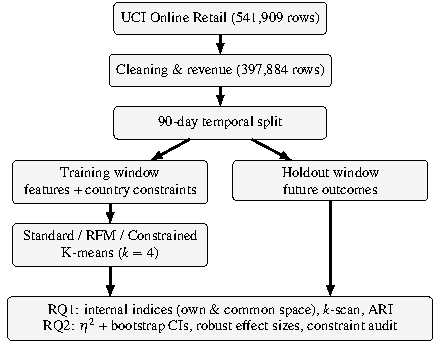
\includegraphics{figures/fig_pipeline.pdf}
\caption{Experimental workflow. Future outcomes are never used to build
features, constraints or clusters.}
\label{fig:pipeline}
\end{figure}

\subsection{Feature engineering}
Table~\ref{tab:features} defines the seven training-window features. Recency
is measured relative to a snapshot one day after the last training
transaction.

\begin{table}[t]
\centering
\caption{Customer-level features computed from the training window.}
\label{tab:features}
\footnotesize
\setlength{\tabcolsep}{3pt}
\begin{tabular}{L{2.2cm}L{4.4cm}c}
\toprule
\textbf{Feature} & \textbf{Definition} & \textbf{Set}\\
\midrule
Recency & Days from last purchase to snapshot date & R, E\\
Frequency & Number of distinct invoices & R, E\\
Monetary & Sum of line revenue & R, E\\
Avg.\ order value & Mean revenue per invoice & E\\
Total units & Sum of quantities purchased & E\\
Product diversity & Number of distinct stock codes & E\\
Mean purchase gap & Mean days between distinct purchase dates (median-imputed) & E\\
\bottomrule
\multicolumn{3}{l}{\scriptsize R = RFM feature set; E = extended feature set.}
\end{tabular}
\end{table}

Given the skew in Table~\ref{tab:desc}, each feature $x$ is clipped at zero,
log-transformed and robustly scaled:
\begin{equation}
\tilde{x} = \frac{\log(1 + x) - \operatorname{median}\!\left(\log(1+x)\right)}
                 {\operatorname{IQR}\!\left(\log(1+x)\right)} .
\end{equation}
Separate scalers are fitted for $\mathbf{X}_{\text{RFM}} \in
\mathbb{R}^{3370\times 3}$ and $\mathbf{X}_{\text{EXT}} \in
\mathbb{R}^{3370\times 7}$.

\subsection{Clustering methods}
\subsubsection{Standard and RFM K-means}
For points $\mathbf{x}_i$ with labels $c_i$ and centroids
$\boldsymbol{\mu}_c$, K-means minimises \cite{macqueen1967some}
\begin{equation}
J_{\text{KM}} = \sum_{i=1}^{n} \lVert \mathbf{x}_i - \boldsymbol{\mu}_{c_i}\rVert^2 .
\label{eq:kmeans}
\end{equation}
Both baselines use scikit-learn \cite{pedregosa2011scikit} with k-means++
seeding \cite{arthur2007kmeanspp}, $k=4$, 20 initialisations and seed 42;
standard K-means is fitted on $\mathbf{X}_{\text{EXT}}$ and RFM K-means on
$\mathbf{X}_{\text{RFM}}$.

\subsubsection{Soft constrained K-means}
With must-link set $\mathcal{M}$, cannot-link set $\mathcal{C}$ and weight
$w \ge 0$, and following the soft-constraint idea of
\cite{basu2004probabilistic}, the constrained model minimises
\begin{equation}
J_{\text{CKM}} = J_{\text{KM}}
 + w\!\left(\sum_{(i,j)\in\mathcal{M}} \mathbb{1}[c_i \neq c_j]
 + \sum_{(i,j)\in\mathcal{C}} \mathbb{1}[c_i = c_j]\right).
\label{eq:ckm}
\end{equation}
Algorithm~\ref{alg:ckm} gives the implementation. It starts from a K-means
solution and sequentially reassigns points (in random order) to the cluster
minimising squared distance plus the penalty for that point's violated
constraints, updating centroids at each step and repairing empty clusters.
The best of four initialisations (maximum 35 iterations) by $J_{\text{CKM}}$
is kept. Constraints are soft, so violation rates are reported as outcomes.

\begin{algorithm}[t]
\caption{Soft constrained K-means (one initialisation)}
\label{alg:ckm}
\footnotesize
\begin{algorithmic}[1]
\Require $\mathbf{X}$, $k$, $\mathcal{M}$, $\mathcal{C}$, weight $w$, $T_{\max}$
\State $\mathbf{c} \gets$ labels from K-means($\mathbf{X}, k$)
\For{$t = 1$ \textbf{to} $T_{\max}$}
  \State $\mathbf{c}_{\text{old}} \gets \mathbf{c}$
  \For{$i$ in a random permutation of $1..n$}
    \State update centroids $\boldsymbol{\mu}_1..\boldsymbol{\mu}_k$ from $\mathbf{c}$
    \For{$c = 1$ \textbf{to} $k$}
      \State $\text{cost}_c \gets \lVert \mathbf{x}_i-\boldsymbol{\mu}_c\rVert^2$
      \State \hspace{1em}$+\, w\,|\{j:(i,j)\in\mathcal{M}, c_j\neq c\}|$
      \State \hspace{1em}$+\, w\,|\{j:(i,j)\in\mathcal{C}, c_j = c\}|$
    \EndFor
    \State $c_i \gets \arg\min_c \text{cost}_c$
  \EndFor
  \State reassign the worst-fitting point to any empty cluster
  \If{$\mathbf{c} = \mathbf{c}_{\text{old}}$} \textbf{break} \EndIf
\EndFor
\State \Return $\mathbf{c}$, $J_{\text{CKM}}(\mathbf{c})$ from \eqref{eq:ckm}
\end{algorithmic}
\end{algorithm}

\subsection{Constraint generation}
No segment labels or expert pairwise judgements exist for this dataset, so
each customer's \emph{modal training-period country} is used as a weak
proxy. Random pairs are drawn; same-country pairs become must-link and
different-country pairs cannot-link until 150 of each are collected (seed
42). No future information is used. Because 90.1\% of customers are British,
\emph{all} 150 must-link pairs are UK--UK and 94\% of cannot-link pairs
contain a UK customer. The 300 pairs touch 544 distinct customers (16.1\%).

\subsection{Evaluation measures}
\subsubsection{Internal validity (RQ1)}
For point $i$ with mean intra-cluster distance $a(i)$ and mean distance to
the nearest other cluster $b(i)$, the Silhouette
\cite{rousseeuw1987silhouettes} is
\begin{equation}
s(i) = \frac{b(i)-a(i)}{\max\{a(i),b(i)\}}, \qquad
S = \frac{1}{n}\sum_i s(i) .
\end{equation}
The Davies--Bouldin index with cluster scatter
$\sigma_c$ and the Calinski--Harabasz index \cite{ikotun2025cluster} with
dispersion matrices $\mathbf{B}_k$, $\mathbf{W}_k$ are
\begin{equation}
\mathrm{DB} = \frac{1}{k}\sum_{c=1}^{k}\max_{c'\neq c}
\frac{\sigma_c+\sigma_{c'}}{\lVert\boldsymbol{\mu}_c-\boldsymbol{\mu}_{c'}\rVert},
\quad
\mathrm{CH} = \frac{\operatorname{tr}(\mathbf{B}_k)}{\operatorname{tr}(\mathbf{W}_k)}
\cdot\frac{n-k}{k-1}.
\end{equation}
Higher $S$ and CH and lower DB are preferred. Each index is computed in the
method's own space and, to remove the representation confound, every
partition is also scored in the other space. Partition agreement is measured
with the adjusted Rand index (ARI) \cite{warrens2022understanding}. To check $k$,
K-means is run for $k=2,\dots,8$ in both spaces.

\subsubsection{Future business separation (RQ2)}
For future outcome $y$ and labels $c$, the correlation ratio
\cite{lakens2013calculating} is
\begin{equation}
\etasq = \frac{\sum_{c} n_c(\bar{y}_c-\bar{y})^2}{\sum_i (y_i-\bar{y})^2},
\label{eq:eta}
\end{equation}
the share of variance in $y$ associated with cluster membership. It is
computed for future revenue, orders, AOV, units and product diversity. Since
\eqref{eq:eta} is sensitive to extreme values, two robust variants are added:
$\etasq_{\log}$, computed on $\log(1+y)$, and the rank-based
$\varepsilon^2 = H/(n-1)$, where $H$ is the Kruskal--Wallis statistic
\cite{fielperes2026effect,virtanen2020scipy}. Uncertainty is quantified with a paired
nonparametric bootstrap \cite{rousselet2021percentile}: customers are
resampled 1,000 times with labels held fixed and the 2.5th and 97.5th
percentiles of each $\etasq$ difference form a 95\% interval. All of these
measures are descriptive associations, not causal or profit effects.

\subsubsection{Constraint satisfaction}
The must-link (cannot-link) violation rate is the share of pairs in
$\mathcal{M}$ split across clusters (in $\mathcal{C}$ placed together). The
same rates are computed for the unconstrained partitions and compared with
the chance rate for a random pair, $1-\sum_c p_c^2$ (must-link) and
$\sum_c p_c^2$ (cannot-link), where $p_c$ are cluster proportions.

\subsection{Sensitivity and robustness}
The constrained model is refitted with $w\in\{0.1, 0.5, 1, 2,
5\}$ (three initialisations, 30 iterations), and constraint sets are
re-sampled with seeds 11, 22, 33, 44 and 55 at $w=1$.


% =====================================================================
\section{Experiments and Results}
\label{sec:results}

\subsection{Experimental setup}
The project notebook was re-run end to end on the original UCI file with
Python 3.13, NumPy 2.5, pandas 3.0, scikit-learn 1.9 and SciPy 1.18, and
extended with the additional analyses described above. All randomness uses
fixed seeds (42 for models, 2026 for the bootstrap). The full pipeline runs
in about 3.5 minutes on a single CPU; the constrained model at $w=1$ took
16~s, and each of its four initialisations converged in 4--5 passes.

\subsection{RQ1: Internal statistical validity}
\label{sec:rq1}

\begin{table}[t]
\centering
\caption{Internal validation at $k=4$ in each method's own feature space
(best in bold).}
\label{tab:internal}
\footnotesize
\setlength{\tabcolsep}{3.2pt}
\begin{tabular}{lccccc}
\toprule
\textbf{Method} & \textbf{$S$\,$\uparrow$} & \textbf{DB\,$\downarrow$} &
\textbf{CH\,$\uparrow$} & \textbf{Min} & \textbf{Max}\\
\midrule
Standard K-means    & 0.3303 & 1.0580 & 1,952.5 & 364 & 1,415\\
RFM K-means         & \textbf{0.3699} & \textbf{0.9705} & \textbf{2,633.6} & 473 & 1,408\\
Constrained K-means & 0.3307 & 1.0590 & 1,949.9 & 349 & 1,428\\
\bottomrule
\end{tabular}
\end{table}

\begin{table}[t]
\centering
\caption{Silhouette and Calinski--Harabasz of every partition scored in
both feature spaces (own-space values on the diagonal in bold).}
\label{tab:cross}
\footnotesize
\setlength{\tabcolsep}{4pt}
\begin{tabular}{lcccc}
\toprule
 & \multicolumn{2}{c}{\textbf{Extended space}} & \multicolumn{2}{c}{\textbf{RFM space}}\\
\cmidrule(lr){2-3}\cmidrule(lr){4-5}
\textbf{Partition} & $S$ & CH & $S$ & CH\\
\midrule
Standard    & \textbf{0.330} & \textbf{1,952} & 0.133 & 882\\
RFM         & 0.162 & 439 & \textbf{0.370} & \textbf{2,634}\\
Constrained & \textbf{0.331} & \textbf{1,950} & 0.135 & 888\\
\bottomrule
\end{tabular}
\end{table}

\textbf{Index ranking.} In own-space scoring (Table~\ref{tab:internal}) RFM K-means is best on all three indices: Silhouette
+0.040, DB $-0.088$ and CH +35\% relative to standard K-means. The ranking,
however, is a property of the representation, not of the partition
(Table~\ref{tab:cross}): scored in the extended space, the RFM partition's
Silhouette falls to 0.162, half that of standard K-means (0.330); scored in
RFM space, standard K-means falls to 0.133. Each method is best in the space
it was optimised for, so own-space indices cannot rank the methods across
representations.


\textbf{Effect of constraints.} Standard and constrained K-means are almost the same
partition: ARI $=0.963$, and after optimally matching cluster labels only
48 customers (1.4\%) are assigned differently. Their indices differ in the
fourth decimal place, and the within-cluster sum of squares rises only from
11,101.9 to 11,111.0 (+0.08\%). The proxy constraints therefore have no
material effect on internal validity. By contrast, standard and RFM K-means
are very different partitions (ARI $=0.381$).

\textbf{Cluster sizes and $k$.} All solutions contain four substantial clusters (349--1,428
customers; Table~\ref{tab:profiles}). A $k$-scan ($k=2,\dots,8$) shows
that the Silhouette is highest at $k=2$ in both spaces and declines
thereafter in the extended space, while in RFM space $k=4$ is a local maximum
($0.370$ versus $0.356$ at $k=3$). $k=4$ is therefore defensible for RFM but
is not Silhouette-optimal for the extended features; $k=2$ separates only
active from lapsed customers, which is of little business use. Future-order
$\etasq$ rises steadily with $k$ (RFM: 0.104 at $k=2$ to 0.306 at $k=8$),
which is why all methods must be compared at the same $k$.


\subsection{RQ2: Future business-metric separation}

\begin{table}[t]
\centering
\caption{Raw $\etasq$ for 90-day future outcomes (best in bold). All
Kruskal--Wallis tests give $p<10^{-100}$.}
\label{tab:eta}
\footnotesize
\setlength{\tabcolsep}{4pt}
\begin{tabular}{lccc}
\toprule
\textbf{Future outcome} & \textbf{Standard} & \textbf{RFM} & \textbf{Constrained}\\
\midrule
Revenue           & 0.0375 & \textbf{0.0405} & 0.0393\\
Order count       & 0.1471 & \textbf{0.1923} & 0.1529\\
Avg.\ order value & 0.00064 & \textbf{0.00137} & 0.00063\\
Units purchased   & 0.0470 & \textbf{0.0515} & 0.0492\\
Product diversity & 0.0829 & \textbf{0.1061} & 0.0846\\
\bottomrule
\end{tabular}
\end{table}

\begin{table}[t]
\centering
\caption{Differences in raw $\etasq$ with paired bootstrap 95\% intervals
(1,000 resamples). $^{*}$Interval excludes zero.}
\label{tab:boot}
\scriptsize
\setlength{\tabcolsep}{2.5pt}
\begin{tabular}{lcc}
\toprule
\textbf{Outcome} & \textbf{Constrained $-$ Standard} & \textbf{RFM $-$ Standard}\\
\midrule
Revenue   & $+0.0018$ $[0.0007, 0.0041]^{*}$ & $+0.0030$ $[-0.0098, 0.0207]$\\
Orders    & $+0.0058$ $[0.0030, 0.0101]^{*}$ & $+0.0452$ $[0.0195, 0.0855]^{*}$\\
AOV       & $-0.000005$ $[-0.0029, 0.0032]$  & $+0.0007$ $[0.0002, 0.0507]^{*}$\\
Units     & $+0.0021$ $[0.0008, 0.0050]^{*}$ & $+0.0045$ $[-0.0058, 0.0214]$\\
Diversity & $+0.0017$ $[-0.0006, 0.0042]$  & $+0.0232$ $[-0.0010, 0.0522]$\\
\bottomrule
\end{tabular}
\end{table}

\begin{table}[t]
\centering
\caption{Outlier-robust effect sizes: $\etasq$ on $\log(1+y)$ and
rank-based $\varepsilon^2$ (Std / RFM / Con).}
\label{tab:robusteta}
\footnotesize
\setlength{\tabcolsep}{3.5pt}
\begin{tabular}{lcc}
\toprule
\textbf{Outcome} & $\boldsymbol{\etasq_{\log}}$ & $\boldsymbol{\varepsilon^2}$\\
\midrule
Revenue   & 0.155 / \textbf{0.227} / 0.158 & 0.190 / \textbf{0.277} / 0.193\\
Orders    & 0.199 / \textbf{0.304} / 0.205 & 0.172 / \textbf{0.263} / 0.176\\
AOV       & 0.129 / \textbf{0.180} / 0.132 & 0.146 / \textbf{0.199} / 0.149\\
Units     & 0.157 / \textbf{0.229} / 0.161 & 0.182 / \textbf{0.263} / 0.186\\
Diversity & 0.145 / \textbf{0.199} / 0.148 & 0.148 / \textbf{0.201} / 0.151\\
\bottomrule
\end{tabular}
\end{table}

\begin{figure}[t]
\centering
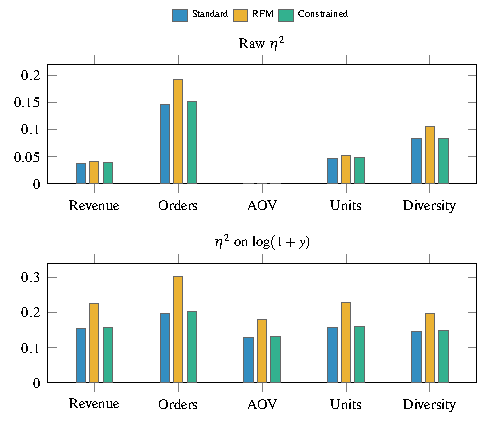
\includegraphics{figures/fig_eta.pdf}
\caption{Share of variance in each 90-day outcome explained by segment
membership, on the raw scale (top) and the log scale (bottom).}
\label{fig:eta}
\end{figure}

\textbf{Raw separation.} RFM K-means has the largest raw $\etasq$ on every
outcome (Table~\ref{tab:eta}, Fig.~\ref{fig:eta}). Future order count is the
most strongly separated outcome (0.192 versus 0.147 for standard K-means).
Constrained K-means exceeds standard K-means on four outcomes by at most
0.006 and is marginally \emph{below} it on AOV.

\textbf{Uncertainty.} The paired bootstrap (Table~\ref{tab:boot}) shows that
the RFM advantage in future orders is clearly larger than sampling noise
(95\% CI $[0.020, 0.086]$), whereas its advantages in revenue and units are
not. Because the constrained and standard partitions share 98.6\% of
assignments, their paired differences have narrow intervals; the
constrained gains in revenue, orders and units therefore exclude zero, but
their upper bounds are at most about 0.010, i.e., about one percentage point of
explained variance. The marginal intervals for individual $\etasq$ values are
wide (e.g., future revenue for standard K-means: $[0.016, 0.082]$), reflecting
the influence of a few very large customers.

\textbf{Robust effect sizes.} Raw $\etasq$ understates segment separation
because a handful of extreme customers dominate the total variance. On a log
scale, or using ranks, segment membership explains 13--30\% of the variance in
every outcome (Table~\ref{tab:robusteta}), roughly three to six times the raw
values for revenue and units. In particular, AOV, which looks unexplained on the raw
scale ($\etasq<0.002$), is moderately separated after the log transform
($\etasq_{\log}$ 0.13--0.18). The ranking of methods is unchanged: RFM is best
on every outcome under both robust measures, and the constrained model adds
at most 0.006 over standard K-means. All Kruskal--Wallis tests are
significant at $p<10^{-100}$, so every method's segments differ in every
future outcome.

\subsubsection*{Segment profiles}
Table~\ref{tab:profiles} profiles the segments, matched across methods by
their training behaviour. All methods find the same four archetypes: a small
high-value group, a regular mid-value group, an occasional or new group and
a large lapsed group of one-time buyers (about 42\% of customers, 37--39\%
of whom returned). The key difference is the high-value segment. RFM's
``champions'' are defined by recency as well as spend (median recency 11 days
versus 23): 93.0\% of them returned in the holdout, compared with 75.8\% for
standard K-means' high-value cluster, and they generated 56.0\% of future
revenue from 14.4\% of customers. The extended feature set weights recency
as one of seven dimensions, so it groups high spenders regardless of how
recently they bought, which explains its weaker separation of future
ordering. The constrained segments are near-copies of the standard ones, and
every segment is 85--93\% British, confirming that country does not structure
the behavioural clusters.

\begin{table*}[t]
\centering
\caption{Segment profiles: training-window medians, holdout return rate,
mean future revenue per customer and share of total future revenue.}
\label{tab:profiles}
\footnotesize
\setlength{\tabcolsep}{3.6pt}
\begin{tabular}{llrrrrrrrr}
\toprule
 & & & & \multicolumn{3}{c}{\textbf{Training (median)}} & \multicolumn{3}{c}{\textbf{90-day holdout}}\\
\cmidrule(lr){5-7}\cmidrule(lr){8-10}
\textbf{Method} & \textbf{Segment} & \textbf{Customers} & \textbf{Share} & \textbf{Recency (d)} & \textbf{Invoices} & \textbf{Spend (\pounds)} & \textbf{Returned} & \textbf{Mean rev.\ (\pounds)} & \textbf{Rev.\ share}\\
\midrule
\multirow{4}{*}{Standard}
 & High-value  & 364   & 10.8\% & 23    & 8 & 2,374 & 75.8\% & 3,556 & 45.4\%\\
 & Regular     & 973   & 28.9\% & 41    & 4 & 1,445 & 73.8\% & 856   & 29.2\%\\
 & Occasional  & 618   & 18.3\% & 51.5  & 2 & 709   & 60.8\% & 459   & 10.0\%\\
 & Lapsed      & 1,415 & 42.0\% & 143   & 1 & 236   & 38.9\% & 312   & 15.5\%\\
\midrule
\multirow{4}{*}{RFM}
 & Champions   & 486   & 14.4\% & 11    & 9 & 3,244 & 93.0\% & 3,285 & 56.0\%\\
 & Regular     & 1,003 & 29.8\% & 71    & 3 & 1,054 & 66.1\% & 577   & 20.3\%\\
 & Recent/new  & 473   & 14.0\% & 15    & 2 & 538   & 59.6\% & 508   & 8.4\%\\
 & Lapsed      & 1,408 & 41.8\% & 155.5 & 1 & 247   & 37.2\% & 310   & 15.3\%\\
\midrule
\multirow{4}{*}{Constrained}
 & High-value  & 349   & 10.4\% & 23    & 9 & 2,438 & 75.9\% & 3,693 & 45.2\%\\
 & Regular     & 968   & 28.7\% & 40    & 4 & 1,463 & 74.4\% & 849   & 28.8\%\\
 & Occasional  & 625   & 18.5\% & 51    & 2 & 712   & 61.1\% & 475   & 10.4\%\\
 & Lapsed      & 1,428 & 42.4\% & 143   & 1 & 239   & 38.8\% & 311   & 15.6\%\\
\midrule
\multicolumn{2}{l}{All customers} & 3,370 & 100\% & 74 & 2 & 566 & 57.0\% & 846 & 100\%\\
\bottomrule
\end{tabular}
\end{table*}

Fig.~\ref{fig:pca} projects the extended features onto two principal
components (87.4\% of variance) \cite{jolliffe2016pca}. Standard and
constrained K-means slice the first component, which is dominated by volume
(frequency, spend, units), into ordered bands; RFM's partition cuts across
these bands because it also separates customers by recency. The narrow
vertical stripe near PC1 $\approx 0.3$ consists of the 1,414 single-purchase-day
customers, whose identical imputed purchase gap collapses their spread; 86\%
of them fall in the lapsed segment, and they make up 86\% of it. Median
imputation therefore shapes the lapsed segment, a limitation noted in
Section~\ref{sec:discussion}.

\begin{figure*}[t]
\centering
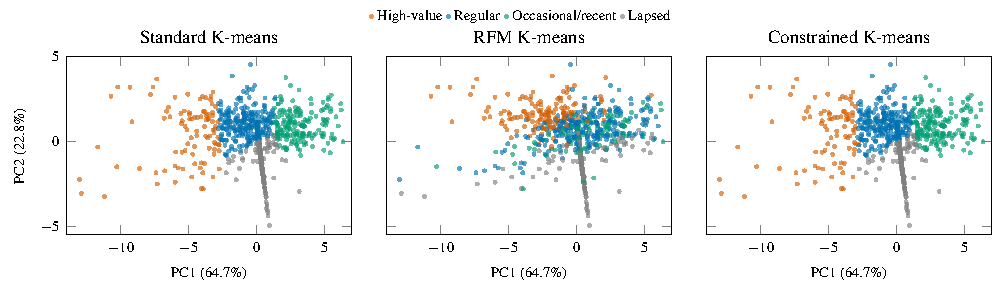
\includegraphics{figures/fig_pca.pdf}
\caption{PCA projection of the extended feature space (random sample of 900
customers), coloured by segment archetype for each method.}
\label{fig:pca}
\end{figure*}

\subsection{Constraint satisfaction and penalty weight}

\begin{table}[t]
\centering
\caption{Violation rates on the 150 must-link (ML) and 150 cannot-link (CL)
country pairs, compared with unconstrained partitions and chance.}
\label{tab:baseline}
\footnotesize
\setlength{\tabcolsep}{3pt}
\begin{tabular}{L{4.2cm}cc}
\toprule
\textbf{Partition} & \textbf{ML violated} & \textbf{CL violated}\\
\midrule
Chance (random pair, standard sizes) & 69.5\% & 30.5\%\\
Standard K-means (no constraints)    & 75.3\% & 30.7\%\\
RFM K-means (no constraints)         & 70.0\% & 27.3\%\\
Constrained K-means ($w=1$)          & 72.0\% & 22.0\%\\
\bottomrule
\end{tabular}
\end{table}

Table~\ref{tab:baseline} shows that the unconstrained standard partition
violates the country constraints at almost exactly the chance rate:
behavioural clusters are unrelated to country. Adding the constraints at
$w=1$ satisfies only five more must-link pairs and 13 more cannot-link pairs
than standard K-means, and the constrained model still violates more
must-link pairs than unconstrained RFM K-means.

\begin{table}[t]
\centering
\caption{Sensitivity of constrained K-means to the penalty weight $w$.}
\label{tab:weights}
\footnotesize
\setlength{\tabcolsep}{2.6pt}
\begin{tabular}{cccccccc}
\toprule
$\boldsymbol{w}$ & \textbf{$S$} & \textbf{DB} & \textbf{ML} & \textbf{CL} &
\textbf{Rev.\ $\etasq$} & \textbf{Ord.\ $\etasq$} & \textbf{ARI}\\
\midrule
0.1 & 0.3314 & 1.058 & 74.0\% & 29.3\% & 0.0392 & 0.1527 & 0.975\\
0.5 & 0.3317 & 1.058 & 73.3\% & 26.7\% & 0.0393 & 0.1530 & 0.970\\
1.0 & 0.3307 & 1.059 & 72.0\% & 22.0\% & 0.0393 & 0.1529 & 0.963\\
2.0 & 0.3282 & 1.063 & 67.3\% & 15.3\% & 0.0393 & 0.1528 & 0.949\\
5.0 & 0.3154 & 1.084 & 48.0\% &  6.0\% & 0.0390 & 0.1510 & 0.918\\
\bottomrule
\multicolumn{8}{l}{\scriptsize ARI is agreement with the standard K-means partition.}
\end{tabular}
\end{table}


Raising $w$ from 0.1 to 5 lowers cannot-link violations from 29.3\% to 6.0\%
and must-link violations from 74.0\% to 48.0\% (Table~\ref{tab:weights}), but lowers the Silhouette from 0.331 to 0.315 and
moves the partition further from the behavioural solution (ARI 0.918).
Future revenue and order $\etasq$ do not improve; both are lowest at $w=5$.
Must-link pairs remain hard to satisfy because UK--UK pairs span the whole
behavioural range of the population, so keeping them together conflicts with
the distance term.

\subsection{Robustness to sampled constraint sets}

\begin{table}[t]
\centering
\caption{Five independently sampled constraint sets ($w=1$). Values below
the standard K-means baseline are marked $\downarrow$.}
\label{tab:robust}
\footnotesize
\setlength{\tabcolsep}{3pt}
\begin{tabular}{lcccccc}
\toprule
\textbf{Seed} & \textbf{$S$} & \textbf{Rev.\ $\etasq$} & \textbf{Ord.\ $\etasq$} & \textbf{ML} & \textbf{CL} & \textbf{ARI}\\
\midrule
11 & 0.3284 & 0.0370$\downarrow$ & 0.1450$\downarrow$ & 56.7\% & 23.3\% & 0.975\\
22 & 0.3309 & 0.0395 & 0.1531 & 64.7\% & 18.7\% & 0.964\\
33 & 0.3281 & 0.0373$\downarrow$ & 0.1467$\downarrow$ & 70.7\% & 22.7\% & 0.972\\
44 & 0.3312 & 0.0393 & 0.1533 & 68.7\% & 24.7\% & 0.964\\
55 & 0.3303 & 0.0392 & 0.1527 & 62.7\% & 18.0\% & 0.961\\
\midrule
Mean & 0.3298 & 0.0385 & 0.1502 & 64.7\% & 21.5\% & 0.967\\
SD   & 0.0014 & 0.0012 & 0.0040 & 5.5\% & 3.0\% & 0.006\\
\midrule
Standard & 0.3303 & 0.0375 & 0.1471 & -- & -- & 1\\
\bottomrule
\end{tabular}
\end{table}

Across five re-sampled constraint sets (Table~\ref{tab:robust}) the
Silhouette and $\etasq$ values are stable, but the direction of the
constrained-versus-standard difference is not: in two of five sets the
constrained model separates future revenue and orders \emph{less} well than
standard K-means. The mean gain in future-order $\etasq$ (+0.003) is smaller
than its across-set standard deviation (0.004). The improvement reported for
the primary constraint set in Table~\ref{tab:boot} is therefore specific to
that sample of pairs rather than a reliable effect of the constraints.

% =====================================================================
\section{Discussion}
\label{sec:discussion}

\subsection{Answer to RQ1}
RFM K-means produced the most compact and best separated clusters on all
three own-space indices, but scoring every partition in a common space
reverses the ranking in the extended space. The internal advantage of RFM is
therefore a property of its three-dimensional representation, not evidence
that it finds better structure. The direct test of constraints, standard
versus constrained K-means in the same space, shows no meaningful difference:
the two partitions agree on 98.6\% of customers. The evidence does not
support a statistical advantage for the tested constrained model.

\subsection{Answer to RQ2}
Constrained K-means did not deliver a reliable improvement in business
separation. Its gains over standard K-means were at most 0.006 in raw
$\etasq$ and 0.006 in $\etasq_{\log}$; it was slightly worse on AOV; the gains
reversed in two of five constraint samples; and stronger enforcement reduced
separation. The improvement that \emph{was} robust came from representation:
RFM segments explained 4.5 percentage points more raw variance in future
orders than standard segments (95\% CI 2.0--8.6) and about 10 points more on
the log scale, because they isolate recently active high-value customers,
93\% of whom bought again.

\subsection{Why the constraints helped so little}
Table~\ref{tab:baseline} gives the main explanation: unconstrained
behavioural clusters already violate the country constraints at the chance
rate, so country carries no information about purchasing behaviour in this
UK-dominated population. In addition, only 16\% of customers are touched by
any constraint, and the soft penalty lets the distance term override most of
them. The result shows that \emph{uninformative} constraints do not help
under \emph{this} heuristic; it does not show that constrained clustering is
ineffective with constraints that encode real behavioural similarity.

\subsection{Measurement and practical implications}
Raw $\etasq$ on heavy-tailed outcomes is dominated by a few customers (the
top 1\% generate 39\% of future revenue), so studies that report it alone may
understate segment usefulness: on the log or rank scale the segments explain
13--30\% of every outcome. In practice, every method isolates a small group
(10--15\% of customers) generating about half of next-quarter revenue, and
recency-aware RFM segments identify the customers most likely to return,
which suits retention targeting. Campaigns based on these segments should
still be tested experimentally, because $\etasq$ measures association, not
response to treatment.

\subsection{Threats to validity}
\begin{itemize}
  \item \emph{External validity:} one retailer, one year and a UK-dominated
  customer base limit generalisation.
  \item \emph{Construct validity:} country constraints are proxies, not
  segment knowledge; revenue excludes returns, costs and margins; 24.9\% of
  rows lack a customer identifier; 42\% of customers have an imputed purchase
  gap, which compresses them into a narrow band of the feature space
  (Fig.~\ref{fig:pca}) and largely defines the lapsed segment.
  \item \emph{Internal validity:} a single 90-day holdout, a fixed $k=4$
  that is not Silhouette-optimal for the extended features, five constraint
  seeds and five weights. Bootstrap intervals hold the partitions fixed and
  so do not include clustering instability.
  \item \emph{Algorithmic:} the custom heuristic is not guaranteed to reach
  a global optimum of \eqref{eq:ckm}.
  \item \emph{Deviation from proposal:} the proposal planned elbow-based
  selection of $k$ and t-SNE \cite{vandermaaten2008tsne}; the final study
  fixed $k=4$ for comparability, reported a $k$-scan instead, and used PCA
  \cite{jolliffe2016pca} for visualisation.
\end{itemize}

% =====================================================================
\section{Conclusion and Future Work}
\label{sec:conclusion}

\subsection{Conclusion}
This study compared standard, RFM-based and soft constrained K-means on the
UCI Online Retail dataset, combining internal validation with a temporal
holdout of future business outcomes. Three findings stand out. First, RFM
K-means scored best on every own-space index, but this advantage is a
representation effect that disappears in a common space. Second, RFM K-means
gave the only robust gain in business separation, explaining substantially
more variance in future ordering than the extended-feature models, because
its segments are defined by recency. Third, country-based constraints changed
the assignment of 1.4\% of customers, were barely better satisfied than by
unconstrained clustering, and produced business-separation gains that were
tiny and reversed across constraint samples. Segmentation should therefore be
judged on validity in a common space, outlier-robust separation of
independently measured outcomes, and constraint satisfaction against an
unconstrained baseline. Constraints help only when they encode real
behavioural knowledge.

\subsection{Future work}
\begin{enumerate}
  \item Replace country proxies with behaviourally meaningful constraints
  (expert pairwise judgements, CRM relationships or shared-basket
  similarity) and measure how many are needed.
  \item Compare the heuristic with COP-KMeans \cite{wagstaff2001constrained}
  and PCKMeans/MPCKMeans \cite{basu2004probabilistic}, reporting objective
  values, convergence and runtime.
  \item Use rolling-origin evaluation over several holdout windows and a
  bootstrap that refits the clusters, so intervals include clustering
  instability.
  \item Select $k$ and $w$ with nested procedures on training data only, and
  add Gaussian mixture, DBSCAN and agglomerative baselines
  \cite{john2023exploration,wani2024comprehensive}.
  \item Test extended feature sets with recency up-weighted, to separate the
  value of additional features from the dilution of recency.
  \item Where data permit, include margins, returns, acquisition cost and
  campaign exposure, and validate segment-based actions with randomised
  experiments.
\end{enumerate}

% =====================================================================
\section*{Reproducibility and Artifact Availability}
The original notebook
(\texttt{Masters\_Constrained\_\allowbreak Customer\_\allowbreak Segmentation\_\allowbreak Experiment.ipynb})
and an extended script (\texttt{run\_analysis.py}) reproduce every number in
this report from \texttt{Online Retail.xlsx} and export all result tables as
CSV files. The project repository is available at
\url{https://github.com/<username>/cos802-constrained-segmentation}
% TODO: replace with the actual repository URL before submission.
and contains a README with run instructions, a \texttt{requirements.txt},
and \texttt{data/}, \texttt{notebooks/} and \texttt{results/} folders. All
randomness uses fixed seeds.

\section*{Acknowledgment}
The author thanks the COS 802 lecturers at the University of Pretoria for
their guidance, and the UCI Machine Learning Repository for making the Online
Retail dataset publicly available.

% =====================================================================
\begin{thebibliography}{99}

\bibitem{chen2012rfm}
D.~Chen, S.~L. Sain, and K.~Guo, ``Data mining for the online retail
industry: A case study of RFM model-based customer segmentation using data
mining,'' \emph{J. Database Marketing \& Customer Strategy Manage.}, vol.~19,
no.~3, pp.~197--208, 2012, doi: 10.1057/dbm.2012.17. [Online]. Available:
\url{https://openresearch.lsbu.ac.uk/item/87978}

\bibitem{salminen2023algorithms}
J.~Salminen, M.~Mustak, M.~Sufyan, and B.~J. Jansen, ``How can algorithms
help in segmenting users and customers? A systematic review and research
agenda for algorithmic customer segmentation,'' \emph{J. Marketing Anal.},
vol.~11, no.~4, pp.~677--692, 2023, doi: 10.1057/s41270-023-00235-5.
[Online]. Available:
\url{https://jyx.jyu.fi/bitstream/123456789/88403/1/s41270-023-00235-5.pdf}

\bibitem{wani2024comprehensive}
A.~A. Wani, ``Comprehensive analysis of clustering algorithms: Exploring
limitations and innovative solutions,'' \emph{PeerJ Comput. Sci.}, vol.~10,
Art.~no.~e2286, 2024, doi: 10.7717/peerj-cs.2286. [Online]. Available:
\url{https://pmc.ncbi.nlm.nih.gov/articles/PMC11419652/}

\bibitem{gomes2023review}
M.~Alves Gomes and T.~Meisen, ``A review on customer segmentation methods for
personalized customer targeting in e-commerce use cases,'' \emph{Inf. Syst.
e-Bus. Manage.}, vol.~21, pp.~527--570, 2023,
doi: 10.1007/s10257-023-00640-4. [Online]. Available:
\url{https://link.springer.com/content/pdf/10.1007/s10257-023-00640-4.pdf}

\bibitem{macqueen1967some}
J.~MacQueen, ``Some methods for classification and analysis of multivariate
observations,'' in \emph{Proc. 5th Berkeley Symp. Math. Statist. Probab.},
vol.~1, 1967, pp.~281--297. [Online]. Available:
\url{https://projecteuclid.org/euclid.bsmsp/1200512992}

\bibitem{christy2021rfm}
A.~J. Christy, A.~Umamakeswari, L.~Priyatharsini, and A.~Neyaa, ``RFM
ranking---An effective approach to customer segmentation,'' \emph{J. King
Saud Univ.---Comput. Inf. Sci.}, vol.~33, no.~10, pp.~1251--1257, 2021,
doi: 10.1016/j.jksuci.2018.09.004. [Online]. Available:
\url{https://doi.org/10.1016/j.jksuci.2018.09.004}

\bibitem{wagstaff2001constrained}
K.~Wagstaff, C.~Cardie, S.~Rogers, and S.~Schr\"{o}dl, ``Constrained K-means
clustering with background knowledge,'' in \emph{Proc. 18th Int. Conf.
Machine Learning (ICML)}, 2001, pp.~577--584. [Online]. Available:
\url{https://www.wkiri.com/research/papers/wagstaff-kmeans-01.pdf}

\bibitem{basu2004probabilistic}
S.~Basu, M.~Bilenko, and R.~J. Mooney, ``A probabilistic framework for
semi-supervised clustering,'' in \emph{Proc. 10th ACM SIGKDD Int. Conf.
Knowledge Discovery and Data Mining}, 2004, pp.~59--68,
doi: 10.1145/1014052.1014062. [Online]. Available:
\url{https://www.cs.utexas.edu/~ml/papers/semi-kdd-04.pdf}

\bibitem{rousseeuw1987silhouettes}
P.~J. Rousseeuw, ``Silhouettes: A graphical aid to the interpretation and
validation of cluster analysis,'' \emph{J. Comput. Appl. Math.}, vol.~20,
pp.~53--65, 1987, doi: 10.1016/0377-0427(87)90125-7. [Online]. Available:
\url{https://core.ac.uk/download/pdf/82326854.pdf}

\bibitem{arthur2007kmeanspp}
D.~Arthur and S.~Vassilvitskii, ``k-means++: The advantages of careful
seeding,'' in \emph{Proc. 18th Annu. ACM-SIAM Symp. Discrete Algorithms
(SODA)}, 2007, pp.~1027--1035. [Online]. Available (Stanford technical
report): \url{http://ilpubs.stanford.edu:8090/778/}

\bibitem{john2023exploration}
J.~M. John, O.~Shobayo, and B.~Ogunleye, ``An exploration of clustering
algorithms for customer segmentation in the UK retail market,''
\emph{Analytics}, vol.~2, no.~4, pp.~809--823, 2023,
doi: 10.3390/analytics2040042. [Online]. Available:
\url{https://doi.org/10.3390/analytics2040042}

\bibitem{ester1996dbscan}
M.~Ester, H.-P. Kriegel, J.~Sander, and X.~Xu, ``A density-based algorithm
for discovering clusters in large spatial databases with noise,'' in
\emph{Proc. 2nd Int. Conf. Knowledge Discovery and Data Mining (KDD)}, 1996,
pp.~226--231. [Online]. Available:
\url{https://cdn.aaai.org/KDD/1996/KDD96-037.pdf}

\bibitem{ikotun2025cluster}
A.~M. Ikotun, F.~Habyarimana, and A.~E. Ezugwu, ``Cluster validity indices
for automatic clustering: A comprehensive review,'' \emph{Heliyon}, vol.~11,
no.~2, Art.~no.~e41953, 2025, doi: 10.1016/j.heliyon.2025.e41953. [Online].
Available: \url{https://pmc.ncbi.nlm.nih.gov/articles/PMC11787482/}

\bibitem{davidson2005clustering}
I.~Davidson and S.~S. Ravi, ``Clustering with constraints: Feasibility
issues and the k-means algorithm,'' in \emph{Proc. SIAM Int. Conf. Data
Mining (SDM)}, 2005, pp.~138--149. [Online]. Available:
\url{https://web.cs.ucdavis.edu/~davidson/Publications/SDM2005Final.pdf}

\bibitem{gonzalez2025semi}
G.~Gonz\'alez-Almagro, D.~Peralta, E.~De~Poorter, J.-R. Cano, and
S.~Garc\'ia, ``Semi-supervised constrained clustering: An in-depth overview,
ranked taxonomy and future research directions,'' \emph{Artif. Intell.
Rev.}, vol.~58, Art.~no.~157, 2025, doi: 10.1007/s10462-024-11103-8.
[Online]. Available: \url{https://doi.org/10.1007/s10462-024-11103-8}

\bibitem{uci2015onlineretail}
D.~Chen, ``Online Retail,'' UCI Machine Learning Repository, 2015.
[Online]. Available: \url{https://doi.org/10.24432/C5BW33}

\bibitem{pedregosa2011scikit}
F.~Pedregosa \emph{et~al.}, ``Scikit-learn: Machine learning in Python,''
\emph{J. Mach. Learn. Res.}, vol.~12, pp.~2825--2830, 2011. [Online].
Available: \url{https://jmlr.org/papers/v12/pedregosa11a.html}

\bibitem{warrens2022understanding}
M.~J. Warrens and H.~van~der Hoef, ``Understanding the adjusted Rand index and
other partition comparison indices based on counting object pairs,''
\emph{J. Classification}, vol.~39, no.~3, pp.~487--509, 2022,
doi: 10.1007/s00357-022-09413-z. [Online]. Available:
\url{https://link.springer.com/content/pdf/10.1007/s00357-022-09413-z.pdf}

\bibitem{lakens2013calculating}
D.~Lakens, ``Calculating and reporting effect sizes to facilitate cumulative
science: A practical primer for t-tests and ANOVAs,'' \emph{Front. Psychol.},
vol.~4, Art.~no.~863, 2013, doi: 10.3389/fpsyg.2013.00863. [Online].
Available: \url{https://pmc.ncbi.nlm.nih.gov/articles/PMC3840331/}

\bibitem{fielperes2026effect}
F.~Fiel Peres, ``Effect sizes for nonparametric tests,'' \emph{Biochem.
Med. (Zagreb)}, vol.~36, no.~1, Art.~no.~010101, 2026,
doi: 10.11613/BM.2026.010101. [Online]. Available:
\url{https://pmc.ncbi.nlm.nih.gov/articles/PMC12701665/}

\bibitem{virtanen2020scipy}
P.~Virtanen \emph{et~al.}, ``SciPy 1.0: Fundamental algorithms for scientific
computing in Python,'' \emph{Nature Methods}, vol.~17, no.~3, pp.~261--272,
2020, doi: 10.1038/s41592-019-0686-2. [Online]. Available:
\url{https://pmc.ncbi.nlm.nih.gov/articles/PMC7056644/}

\bibitem{rousselet2021percentile}
G.~A. Rousselet, C.~R. Pernet, and R.~R. Wilcox, ``The percentile bootstrap:
A primer with step-by-step instructions in R,'' \emph{Adv. Methods Pract.
Psychol. Sci.}, vol.~4, no.~1, 2021, doi: 10.1177/2515245920911881.
[Online]. Available: \url{https://doi.org/10.1177/2515245920911881}

\bibitem{jolliffe2016pca}
I.~T. Jolliffe and J.~Cadima, ``Principal component analysis: A review and
recent developments,'' \emph{Phil. Trans. R. Soc. A}, vol.~374, no.~2065,
Art.~no.~20150202, 2016, doi: 10.1098/rsta.2015.0202. [Online]. Available:
\url{https://doi.org/10.1098/rsta.2015.0202}

\bibitem{vandermaaten2008tsne}
L.~van~der Maaten and G.~Hinton, ``Visualizing data using t-SNE,''
\emph{J. Mach. Learn. Res.}, vol.~9, pp.~2579--2605, 2008. [Online].
Available: \url{https://jmlr.org/papers/v9/vandermaaten08a.html}

\end{thebibliography}

\end{document}
